%% This is an example first chapter.  You should put chapter/appendix that you
%% write into a separate file, and add a line \include{yourfilename} to
%% main.tex, where `yourfilename.tex' is the name of the chapter/appendix file.
%% You can process specific files by typing their names in at the 
%% \files=
%% prompt when you run the file main.tex through LaTeX.

%\makeglossaries
\newacronym{utm}{UTM}{Unmanned Aircraft System Traffic Management}
\newacronym{uav}{UAV}{Unmanned Air Vehicle}
\newacronym{uas}{UAS}{Unmanned Aircraft System}
\newacronym{nas}{NAS}{National Air Space}
\newacronym{fpv}{FPV}{First Person View}
\newacronym{vll}{VLL}{Very Low Level}
\newacronym{sme}{SME}{Small and Medium Enterprise}
\newacronym{tcas}{TCAS}{Traffic Collision Avoidance System}
\newacronym{gcs}{GCS}{Ground Control Station}
\newacronym{icao}{ICAO}{International Civil Aviation Organization}
\newacronym{faa}{FAA}{Federal Aviation Administration}
\newacronym{nasa}{NASA}{National Aeronautics and Space Administration}
\newacronym{easa}{EASA}{European Aviation Safety Agency}

\chapter{State of the Art}

This chapter includes the current status of a variety of topics.
Integration of unmanned systems into airspace is the first to be discovered in the course of this chapter since it constitutes the motivation for this thesis.
Then as a mitigation measure to achieve safe integration of drones into airspace, fault tolerant control systems have been visited with a focus on fault detection and diagnosis.
The rise of machine learning methods in the last decade is referred finally, since it is utilized to diagnose faults in this study.

\section{Integration of Drones into Airspace}

Commercial advantages offered by drones are already targeted by big companies worldwide. 
The airspace regulatory authorities seem to be squeezed in between the companies, demanding a fast as possible access to airspace, and the concerns of the public about potential privacy breaches, 
safety and liability issues \cite{droneDisasters,droneImageProblem}. 
Even with today's strictly regulated airspace, reported occurrences show that there are hurdles to solve before a further integration of \gls{uas} to airspace.

With Riga Conference\footnote{The Future of Flying, Conference on remotely piloted aircraft systems, Riga, 6 March 2015} in 2015, Europe has entered a path towards a unified regulatory framework design to allocate airspace with a growing number of drones. 
Its diversity, innovation, and international structure is offering huge potential for new jobs. 
EASA (European Aviation Safety Agency) has been assigned by European Commission to develop two main aspects:

\begin{itemize}
\item{EU Regulatory Framework for drone operation}
\item{Proposals for the regulation of low-risk drone operations, key elements of the future Implementation Rules (IRs)}
\end{itemize}


With a starting point in Riga Declaration \cite{rigaDeclaration}, and building up on Regulations (EC) No 216/2008 (Basic Regulation) \cite{basicRegulation}, A-NPA (Advance Notice of Proposed Amendment) \cite{A_NPA_EASA2015} introduces three main category of operations and asks for a public consultation. 
This consultation period has already over, but to see how these reviews are accounted for in the Technical Opinion \cite{technicalOpinion}, the Explanatory Note of the opinion can be referred.
In the report, drones are grouped under two main categories; remotely piloted and autonomous. 
An autonomous drone, defined by ICAO (International Civil Aviation Organization) \cite{ICAO_RPASmanuel} as: A drone that does not allow pilot intervention in the management of the flight. 
Aside sounding like science fiction, one of the reasons that EASA has switched to using the term drone and categorize it (remotely piloted or autonomous) rather than using UAS or RPAS to point the system, is to ensure a fast growing development of autonomy of drones.

\begin{figure}
\begin{center}
%\includegraphics[width=11.3cm]{figures/FTCmethods}    % The printed column width is 8.4 cm.
\includegraphics[width=11.3cm]{figures/mermaid_statue_drone}
\caption{Statue of mermaid in Riga handling airspace (for fun)} 
\label{fig:mermaid_statue_drone}
\end{center}
\end{figure}


While mentioning the efforts by different organizations to accommodate drones in airspace, let's look at the present regulatory context from european and international perspectives.
ICAO is a United Nations Organization working with 191 Member States of Chicago Convention (Convention on International Civil Aviation) and global aviation organizations. 
For now, international circulation of drones are not allowed by Article 8 of Chicago Convention \cite{chicagoConvention}. 
Starting from 2003, ICAO starts to study on Standards and Recommended Practices (SARPs) on drones, to which member states will refer when developing their legally enforceable national civil aviation regulations. 
2018 is the proposed year for draft SARPs with a focus on international drone operations. 
Until then, the work of ICAO can be traced by studies of UAS Study Group (set up by ICAO in 2007), which developed Circular 328 AN/190 on Unmanned Aircraft Systems \cite{ICAO_Circular}, an amendment to Annex 2 (Rules of the Air) \cite{amendment43toAnnex2} and to Annex 7 (Aircraft Nationality and Registration Marks) \cite{amendment6toAnnex6}.
From European perspective, Basic Regulation (Regulation EC No.216/2008) \cite{basicRegulation} is the one holds right now. 
Its Article 2 and Annex II limit the regulation to apply to only drones with a maximum take off mass above 150 kg and/or except operations on military, customs, police, firefighting, search and rescue, and experimental work. 
Those that are not covered by Basic Regulation are handled by national aviation legislations, which are not really harmonized and mostly designed with an assumption that small drones are operating locally.
EASA is working on different aspects of drone integration into airspace. 
Last year, EASA published the `Prototype' Commission Regulation on Unmanned Aircraft Operations \cite{prototypeRegulation}, after an public consultancy with A-NPA 2015-10 (Advance Notice of Proposed Amendment) \cite{A_NPA_EASA2015} and its resulting Opinion \cite{technicalOpinion} with an Explanatory Note of Opinion. 
Another work from EASA aims to authorize general principles for the type certification for fixed wing and helicopter drones separately utilizing a policy adopted by agency in 2009 (E.Y013-01) \cite{EY013_01policyStatementAirworthinessCertification}.

In the proposed regulation by EASA, an operation and risk centric categorization has been followed. 
\emph{Open}, \emph{specific}, and \emph{certified} are the three categories proposed corresponding to different risk levels they possess.

\begin{itemize}
\item{\textbf{Open Category} encompasses low risk operations, like most of leisure flights and some professional activities. 
Operations falling in this category do not require an explicit authorization from civil aviation authorities. 
But, they are subject to strict operational limitations (e.g., no proximity to people, traffic, infrastructures; no dangerous items; one pilot per UAS; no item dropping). 
These operational limitations are sufficient to mitigate the low risk. 
Though some professional activities fit in this category, the main goal is to regulate leisure types of operations \cite{manfredi2018unmanned}.}
\item{\textbf{Specific Category} regroups medium risk operations, such as operation beyond visual line of sight (i.e., no visual contact between pilot and UAV during flight). 
To facilitate the regulation process, a set of scenarios with specific operational limitations are designed. 
To operate within a scenario, the UAS needs to comply with a list of requirements.
For operations outside the scope of the scenarios, a risk analysis must be carried out to show that the existing risks are properly mitigated. 
To facilitate this risk analysis process, JARUS developed a framework called the Specific Operations Risk Assessment (SORA). 
SORA considers threats, which contribute to the risk, and barriers, which mitigate the risk, to evaluate the actual risk of an operation and decide if the resulting mitigated risk is low enough to allow the operation as illustrated in Fig.~\ref{fig:sora_barriersSmallerVersion}.
The risk analysis needs to be validated by the authorities in order to authorize an operation not included in the standard scenarios \cite{manfredi2018unmanned}.}
\item{\textbf{Certified Category}  Operations with risk that cannot be mitigated in \emph{Specific Category} are evaluated in \emph{Certified Category}. 
These represent high risk operations, for example large cargo delivery in urban areas. 
These are likely to be operations with a risk close to current manned aviation. 
As such, the aircraft, avionics, pilot/crew and operator will need to be certified in order to fly these operations. 
The fact that a certification process is involved increases the complexity of the introduction of UAS in these types of operations. 
Indeed, before being able to certify a piece of equipment, a standard must be developed for this equipment. 
Standardization can be understood as the process of defining details and minimum requirements for safe and uniform operation across a diverse range of implementations. 
However, as of today, not all the parts required to fly a UAS have corresponding standards, e.g., Detect And Avoid (DAA) systems, C2 links, pilot training. 
So, enabling this category of operation requires extra effort and time for the industry to agree on standards. 
For \emph{Certified Category}, harmonization at the ICAO is planned to allow international operations \cite{manfredi2018unmanned}.}
\end{itemize}
 
\begin{landscape}
\begin{figure}
\begin{center}
\includegraphics[width=24cm]{figures/sora_barriersSmallerVersion}    % The printed column width is 8.4 cm.
\caption{SORA structure: threats, threat barriers, hazard, harm barriers, harms} 
\label{fig:sora_barriersSmallerVersion}
\end{center}
\end{figure}
\end{landscape}


\begin{figure}
\begin{center}
\includegraphics[width=9cm]{figures/USpacePortable}    % The printed column width is 8.4 cm.
\caption{U-space illustration \cite{UTMairspace}} 
\label{fig:USpacePortable}
\end{center}
\end{figure}

Latest efforts for the integration of drones into airspace, welcomed a relatively new concept called the `U-Space'. 
This approach has been injected to immediate plans at European level, to accommodate drones in urban areas. 
While EASA is searching for solutions for the integration of drones in a variety of presumed airspaces, commissioner Violeta Bulc mentions other pillars in high level conference\footnote{Drones as a leverage for jobs and new business opportunities} in Warsaw. 
She offers that in parallel to the efforts of EASA, two other pillars has to be tackled, UTM (UAS Traffic Management) and the U-Space.
U-Space covers the usage of drones especially in U-rban areas and equal share of airspace, in which case `\emph{U}' stands for `\emph{you}'.
To point out its availability to everyone, the services available through a portable phone is illustrated as in Fig.~\ref{fig:USpacePortable}.
The sympathetic name riddles seem to be the search of public acceptance for drones in urban areas.
The goals are highly challenging and given as \cite{UTMairspace}

\begin{itemize}
\item{``Safe: safety at low altitude levels will be just as good as that for traditional manned aviation. The concept is to develop a system similar to that of Air Traffic Management for manned aviation.''}
\item{``Automated: the system will provide information for highly automated or autonomous drones to fly safely and avoid obstacles or collisions.''}
\item{``Up and running by 2019: for the basic services like registration, e-identification and geo-fencing. However, further U-Space services and their corresponding standards will need to be developed in the future.''}
\end{itemize}

EASA regulations already covering the airspace issued in U-Space, either under specific or certified categories (depending on the risk of the operation). 
By pointing the U-Space, a faster integration is prospected in urban areas.
It seems we are not far from the images of flying vehicles populating the sky as such in fictions. 
Even better then imagined, this time, without drivers and more automated. 

\begin{figure}
\begin{center}
\includegraphics[width=17cm]{figures/amazonDroneOperations}    % The printed column width is 8.4 cm.
\caption{Airspace design for small drone operations by Amazon \cite{amazonAirspace}} 
\label{fig:amazonDroneOperations}
\end{center}
\end{figure}

In US, to tackle the safety challenges and help the regulation development, NASA is currently carrying out a four years research program (up to 2019) to enable Unmanned aircraft traffic management solutions which are structured yet flexible when needed. 
To ensure safety, this integration needs to be achieved through airspace management and UAS reliability.
Also, preliminary airspace designs, like the one proposed by Amazon shown in Fig.~\ref{fig:amazonDroneOperations}, identify different zones depending on the UAS capabilities, population density and altitude. 

United Arab Emirates (UAE) accelerates the safe integration of drones into urban airspace, by settling and agreement for UAS Traffic Management (UTM) with Nokia as part of its `Next generation network for mission-critical and smart city services' \cite{nokiaDubai}.
Aiming tracking/managing all drones in the airspace, Nokia is offering solutions for automated flight permissions, no-fly zone regulation, beyond visual line of sight (BVLOS) safety operations utilizing LTE protocols for low latency, reliable and resilient communication. 
For compatibility with this system, drones will be equipped with LTE dongles, and access modules for telemetry data access.



\iffalse
\subsection{Certification of analytical approaches NOT FINISHED }\label{ch2:certificationOfAnalyticalApproaches}

Due to the lack of the modeling for interaction in-between different FPE  (Flight Parameter Estimation), FDD and FTC modules in simulations, leaves them free from practical limitations, offering a long way to go for these analytical methods to be certified. 

[REF : certificationOfFDD]
[REF : clearanceOptimBased]


safety issues

http://www.techrepublic.com/article/12-drone-disasters-that-show-why-the-faa-hates-drones/

%FP7_RECONFIGURE REF : FP7RECONFIGUREgeneral page : 978 starting with 4 980 section 4. VERIFICATION AND VALIDATION

Regulations EU : https://easa.europa.eu/unmanned-aircraft-systems-uas-and-remotely-piloted-aircraft-systems-rpas

The increased cost will be inevitable for the demands of certification. REF : UAVreliabilityStudy

This increment could be even beyond expectations that it could lead to a cancellation of project:  REF : http://www.defenseindustrydaily.com/euro-hawk-program-cleared-for-takeoff-03051/

Regulations US : 

US Delivery Drones (News from Guardian http://www.theguardian.com/technology/2015/nov/06/alphabet-and-facebook-compete-with-secret-drone-plans)
--------------------
Even if the companies solve the technical challenges of keeping drones aloft for long periods, sharing data via lasers and serving city-sized areas, both Alphabet and Facebook still face regulatory hurdles. Neither company has been granted a waiver to the current FAA blanket ban on the commercial operation of unmanned aircraft.

Alphabet has applied for an exemption, called ?333? after a section of the FAA regulations, for its Project Wing delivery drones, but that is yet to be granted and in any case would only clear operation to a maximum height of 400ft. Google has also been testing its delivery drones in the US under a Certificate of Waiver or Authorization (COA) with Nasa, which permitted flights intended to help Nasa develop an automated air traffic control system for low-flying drones. This would not apply to drones flying far above other manned and unmanned aircraft.

?There?s not a lot to run into between 60,000 and 90,000 feet,? says Cummings. ?But I?m sure regulators would be deeply suspicious if Google and Facebook were flying these over the US.?

Facebook and Alphabet would not comment.

What's really standing in the way of drone delivery?
---------------------------------------------------------
http://www.theverge.com/2016/1/16/10777144/delivery-drones-regulations-safety-faa-autonomous-flight
\fi


\section{Paparazzi Autopilot in Relation with the New Autopilot}

\subsection{Introduction}

\subsection{Open Source Systems in Relation with the New Regulatory Context}

To tackle the safety challenges and help the regulation development, NASA is currently carrying out a four years research program (up to 2019) to enable Unmanned aircraft traffic management solutions which are structured yet flexible when needed. 
To ensure safety, this integration needs to be achieved through airspace management and UAS reliability.

The preliminary airspace designs, like the one proposed by Amazon, identify different zones depending on the UAS capabilities, population density and altitude. 
Plus, different national rules and their progressive refinement pushes to cope with a variety of requirements. 
Open source and modular architectures are key to adapt these requirements. 
As such, NASA's UTM builds, later to be refined by FAA, discusses modularity to be essential for UAS software to follow their evolution. 

Concerning reliability, current regulations focus on flight constraints but they might be expected to involve regulations on software and hardware components as well. 
In such case, the increased cost will be inevitable for the demands of certification. 
This could put too many constraints on UAS manufacturers who desire to access the some specific regions of airspace. 

In Europe, Regulation (EC) No 216/2008 mandates the European Aviation Safety Agency to regulate Unmanned Aircraft Systems (UAS) and in particular Remotely Piloted Aircraft 
Systems (RPAS), when used for civil applications and with an operating mass of 150 Kg or more.

\section{UAVs populating airspace}\label{ch2:certificationOfAnalyticalApproaches}



Advent of the new era of \gls{uas} seems to be hold by an unseen barrier of lack of 
regulatory framework for now. Different institutions all over the world, specifically \gls{nasa} 
and faa in US, easa in Europe and international bases such as \gls{icao} are addressing 
safe integration of \gls{uas} in airspace. Although the approaches of regulatory bodies 
may vary, the aim remains the same: safe integration as soon as possible. 

The tackles of safety during integration of \gls{uas} to airspace refer to different technical 
and organizational aspects including but not limited to control of traffic in segregated and 
non-segregated airspace, reliable communication, robust control of the \gls{uav}, trajectory planning, detect\&avoid.


\section{Modularity}\label{ch2:modularity}

The current evolving nature of regulations and the variety of organizations in charge 
of the airspace rule making calls for flexible solutions to cope with these fruitful environments. 

\subsection{Airspace Categorization}
The \gls{uas} in the \gls{nas} project points to a performance-based routine access to 
all segments of the national airspace for all unmanned aircraft system classes, after the 
safety and technical issues are addressed thoroughly. As a start, \gls{nasa} and faa 
seem to have a short term goal to integrate \gls{uas} in low-altitude airspace as early 
as possible. They further aim to accommodate increased demand safely, efficiently in 
the long term. \gls{nasa} and faa seem to handle the airspace above 500 feet and the 
one below separately. easa, tasked by the European Union, is planning a risk based approach, 
accommodating the \gls{uas} in the airspace under three different categories, low risk, 
specific and high risk. Both regulators seem to categorize the airspace and scale regulatory 
needs according to some criteria. To answer different needs of different categories, flexibility 
given by the high level of modularity of open source autopilot systems will be a handy tool. 

\subsection{National Regulations}
Circulation of \gls{uas} internationally is somewhat prevented by the Chicago convention 
unless an agreement holds between Contracting States \cite{A_NPA_EASA2015}. \gls{icao} is aiming 
to develop international standards and recommended practices to which the member states 
could refer to when developing their national civil aviation regulations. Even though a similar 
base is aimed, national aviation legislations will not be the same because of the different 
expectations of nations about \gls{uas} aviation. 

\subsection{Accommodating evolution of regulations}
Prescriptive rules seem to cause some difficulties since the technical area on \gls{uas} 
systems develop rapidly \cite{A_NPA_EASA2015}. Innovations both on the aircraft and the operation 
type of \gls{uas} will accelerate especially after the regulations are set. Thus, regulatory 
bodies call for refinable operational requirements and system architectures to evolve into 
a safer and efficient integration of \gls{uas} into airspace. The systems to cope with the 
regulations should also be modular and flexible in order not to be superseded by the 
innovations in the area. 
Thus, the aviation regulatory bodies aim to achieve designs with flexibility where possible, 
structure where needed. Having flexible hardware and software points to modularity, which 
is pretty much best supported via open source systems.



\section{Reliability}\label{ch2:reliability}

Improvement of the reliability of the flight is considered to be one of the main goals for 
integrating military \gls{uav}s into civil airspace according to Unmanned systems roadmap 
by US Office of the Secretary of Defense, DoD \cite{UnmannedSystemsRoadmapDoD}. 
Compared to manned counterparts, \gls{uav}s experienced failures with a frequency of two 
orders of magnitude more in the military domain.  Although this changed last years with 
the technological improvements, making the \gls{uav}s as reliable as early manned military 
aircraft, it seems not enough from the DoD perspective. This can be realized by checking 
the biggest chunk of control technologies budget for research and development, which is 
health management and adaptive control.

To achieve a safe flight is not an easy task considering the unknowns of the systems hardware, 
environment and possible system faults and failures to emerge. Also, increasing demand on 
cost effective systems, resulting in smaller sensors and actuators with less accuracy, 
impose the software to achieve even more. The expectation that \gls{uav}s should be less 
expensive than their manned counterparts might have a hit on reliability of the systems. 
Cost saving measures other than the need to support a pilot/crew onboard or decrement 
in size would probably lead to decrease in system reliability. 

\subsection{\gls{sme}s and Certification Costs}

Utilizing drones for quicker and cheaper deliveries could be rewarding for \gls{sme}s 
since cost per mile of a drone is less then 1 / 30 of the average diesel truck. Being an 
early bird might put the \gls{sme}s in an advantageous position, considering the increase 
in the capabilities of the drones with inevitable acceleration thrusted by research activities 
and their widened application areas. 

Nevertheless, the fairly cheap access to drones and their relatively cheap utilization cost 
does not seem to be enough to put them to air right now due to the heavy cost of certification 
and regulatory hurdles \cite{UAVreliabilityStudy}. In this concern, capable open source solutions 
could be a good way to loosen the tie.  Otherwise, \gls{sme}s, an important factor in drone 
business might not survive. Even worse, they might operate them without relevant permission, 
scarifying a substantial fine as reported by Civil Aviation Authority (CAA). This will compromise 
security in the system contradicting the hopes for reliable integration of drones into airspace. 

\subsection{Individuals and Education}

Individuals, as well as \gls{sme}s, suffer from the same budget constraints. Personal \gls{uav} 
usage counts for a substantial amount of the drone ecosystem.  Both US and European 
authorities mention the importance of individuals in utilizations of drones. There is a community 
with a passion of aviation and potential, but most probably not very experienced.  

\subsection{Flight Heritage for Risk Assessment}

Drone industry being extremely innovative, technical developments could supersede the 
prescriptive rules as regulations. Thus a solution might be to follow a risk based approach 
rather that to have strict rules to cope with. Predicted regulations in Europe seems to evolve 
under different categories dedicated to specific operation risks. Flight heritage and occurrence 
reporting is expected to be an inevitable part of safety risk assessment to achieve reliable flight. 

\subsection{Support for real time planning and onboard vehicle automation}
To access low-altitude airspace with the use of small unmanned aircraft safely, an important 
ability could be to implement real-time planning and on-board vehicle automation. Amazon 
offers that this approach will allow some flexibility to adapt to variable situations such as 
weather changes, severe winds or any other emergency needs.

To conclude, the introduction of \gls{uas}s in the \gls{vll} airspace comes with numerous challenges. 
Though various ways to address them have been proposed, there is still no certainty about how it will be done in the end.

One sure thing is that it will involve two main actors: \gls{utm} and \gls{uas}s. This work focused on the later.	


\section{Fault Tolerant Control Systems}

Improvement of the reliability of the flight is considered to be one of the main obstacles for integrating UAVs into civil airspace. 
To achieve a safe flight is not an easy task considering the unknowns of the systems, environment and possible system faults and failures to emerge. 

\subsection{Loss of Control in Aviation}

One of the biggest contributors to fatal accidents is considered as aircraft \emph{loss of control} (LOC). 
Joint Safety Analysis Team (JSAT) defines LOC as an ``significant, unintended departure of the aircraft from controlled flight, the operational flight envelope, or usual flight attitudes, including ground even'' where \emph{significant} refers to events resulting with an incidence or accident \cite{russell2000joint}. 
Control failures, inappropriate pilot action (inaction) in a healthy aircraft, and vehicle impairment are examples of LOC events \cite{richards2016vehicle}.

LOC-I (loss of control in-flight) is defined as ``an extreme manifestation of a deviation from intended flight path'' and is the most deadly accident type with 37 fatal accidents per year (for fixed-wings) \cite{easa:LOC}.
Although LOC-I is the cause behind many fatal accidents, manned aviation have a very limited use of LOC prevention and recovery \cite{belcastro2017aircraft}. 
Having no single action to prevent LOC events, technical limits in LOC simulations such as full stall or failure simulations, constitute some of the challenges on the way to LOC event prevention and recovery solutions.

To offer prevention strategies, the causes of LOC accidents and upsets should be studied thoroughly. 
LOC events have been categorized by Ref.\cite{lambregts2008airplane} under five main topics, two of them being the most common. 
Aerodynamic stall and flight control system are the biggest factors that led to LOC accidents and upsets in 15 years log of LOC accidents in transport airplanes.
Autopilot commands and control surface failures are considered under flight control failures category, the second most fatal LOC of all types \cite{lambregts2008airplane}. 
The same study also shows that, the percentage if flight control system upset incidents among other LOC events has risen from 9\% to 22\% after 1993 (Pre-1993 compared to 1993-2007).
An educated guess for the reason behind this could be increased complexity of onboard systems suppressing the technological advancements in fault detection and recovery. 
Thus addressing onboard fault detection and recovery could contribute to reduce the likelihood of LOC accidents and/or fatalities. 
The importance of those emergency recovery measures are magnified for unmanned systems considering the number of drones in the airspace will eventually increase, and difficulties inherent in unmanned systems. 

Unmanned systems are more susceptible to LOC events they are less robust to disturbances and recovery must be held by the onboard computer or a remote pilot\cite{richards2016vehicle}.
Studies for drone regulations accelerated the pace for the assessment of risk for drone operations. A recently published \emph{Annual Safety Review 2017} \cite{annualSafetyReview} discusses the aviation accidents in detail containing a chapter specialized for drones. 
This report by EASA, involves the data from European Central Repository (ECR) experienced by EASA member states.
With the increase in the number of drones and possibly raising consciousness on reporting occurrences, the numbers of non-fatal accidents raised by 470\% in 2016 relative to 2011-2015 average, luckily maintaining zero fatalities. 
Most of the times, it is commercial airliner pilots to report the occurrences, and rarely the UAS pilot.
The prior key risk areas has been investigated and aircraft upsets is by far the most common cause of the occurrences and set as the first key risk to address for safe integration of drones into airspace. 
50\% of RPAS accidents falls in this case which often results in a damage or destruction of UAS following loss of the control of the drone by the pilot.
Second key risk area is airborne collision although it is rarely encountered due to probable frequency with exponential increase in the number of drones. 
Obstacle collision is the 3rd risk area which will tend to increase with integration of drones especially in urban areas.

Designing recovery measures for unmanned systems has further challenges due to lack of redundancies utilized in manned aviation and use of cheaper and less accurate components.
Introducing intelligent algorithms to reduce the risk of harm is usually adopted for those systems which are limited in hardware. 
Fault tolerant control systems (FTCS) are designed to issue solutions to systems which are under fault/failure. 
There are a wide range of different strategies offered for this solution such as passive or active FTCS, where the latter requires a fault detection and diagnosis (FDD) phase \cite{ducard2009fault}. 
FDD methods are used to find out if there is any fault/failure in the system and the kind of the fault. 

After the fault is known, an assessment of the current abilities of the drone is vital. 
The severity of the situation should be evaluated to decide if a recovery is viable. 
If it is, current situation of the drone should be considered during the design of recovery control methodologies.
In the case a recovery is likely to fail, a safe ditch maneuver can abruptly decrease the number of fatalities. 
Maps pointing zones with no or minimum population could be uploaded onboard and the safest region to ditch can be selected. 
Since those situations are handled by the pilot for manned aviation, the number of works to assess and plan ditch maneuvers is very few for unmanned systems. 
NASA is offering \emph{Safe2Ditch} \cite{nasa:safe2ditch} to offer autonomous crash management yet it is at design stage now. 


\subsection{FTCS Terminology}\label{ch2:terminology}

Systems are often susceptible to faults of different nature. 
Existing irregularities in sensors, actuators, or controller Fig.~\ref{fig:faultsInTheSystem} could be amplified due to the control system design 
and lead to failures. 
A fault could be hidden thanks to the control action \cite{ducard2009fault}.

\begin{figure}
\begin{center}
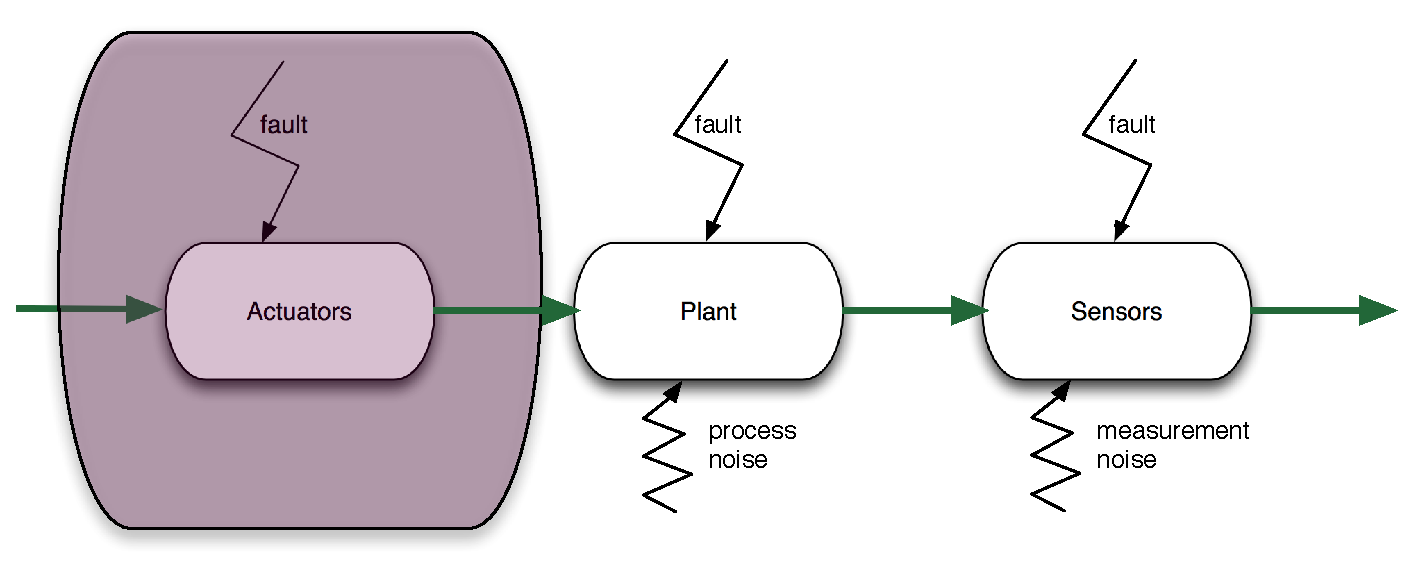
\includegraphics[width=15cm]{figures/faultsInTheSystem}    % The printed column width is 8.4 cm.
\caption{Faults altering the system } 
\label{fig:faultsInTheSystem}
\end{center}
\end{figure}

Since fault tolerant control is comprised of a set of different disciplines and a relatively new topic, the terminology is not solid. 
FDI could be a proper example to this ambiguity. 
In some works, it stands for Fault Detection and Isolation while in some other Fault Detection and Identification, which could also named after Fault Detection and Diagnosis, 
meaning that identification is added to Fault Detection and Isolation \cite{zhang2008bibliographical}.

One of the first attempts to unify the terminology is carried out by IFAC SAFEPROCESS technical committee in 1996 and published by \cite{isermann1997trends}. 
Fault, failure, and the methodology to handle those such as fault detection, fault isolation, fault identification, fault diagnosis and supervision terms explained separately to avoid the ongoing ambiguity 
in this field. 
Although fault detection methods are clearer in the work, difference between the methods for two steps of fault diagnosis, namely the fault isolation and fault identification is not very obvious.

\subsection{Conventions for a Safe Flight}\label{ch2:conventions}

The widely used method to increase reliability is to use more reliable components and/or hardware redundancy. 
Both requires an increase in the cost of the UAS conflicting one of the main reasons of UAS design itself band consumer expectations 
\cite{angelov2012sense}. To offer solutions for all different foreseen categories of 
airspace, a variety of approaches should be considered. While hardware redundancy 
could cope with the failure situations of UAVs in the certified airspace, it may not be 
suitable for UAVs in open or some subsets of specific categories due to budget 
constraints. Analytical redundancy is another solution, may be not as effective and 
simple as hardware redundancy, but relies on the design of intelligent methods to 
utilize every bit of information onboard aircraft wisely to deal with the instances.  

There are three approaches to achieve safe FTC in standard flight conventions. 
First one is the fail operational systems which are made insensitive to any single 
point component failure. The second approach is the fail safe systems where a 
controlled shut down to a safe state is practiced whenever a critical fault is pointed 
out by a sensor. The level of degradation assures to switch to robust (alternate) or 
direct (minimal level of stability augmentation independent of the nature of the fault) mode. 
Switching from nominal mode to the robust and direct modes leads to a decrease 
in the available GNC functions. This causes a degradation in ease of piloting. And 
also some optimality conditions could have been compromised. The third approach 
is fault tolerant control systems in which redundancy in the plant and the automation 
system is employed to design software that monitors the components and takes in 
action whenever needed. The strategy is most probably to try to keep plant availability 
and accept reduced performance \cite{blanke2000fault}.

RECONFIGURE project of FP7 \cite{goupil2015overview} aims to attack at this 
problem of piloting degradation and optimality compromisation by attacking 
Flight Parameter Estimation (FPE) which is the online estimation of aircraft parameters, 
FDD and FTC in case of off-nominal events \cite{RECONFIGURE} They utilize a black 
box nonlinear model of aircraft and The project uses some outputs of a previous FP 7 
project ADDSAFE leaded by Deimos Space \cite{ADDSAFE}.

\subsection{Methods for Fault Tolerant Control Systems}\label{ch1:methodsFTCS}

Among different categorizations for the fault tolerance, there are options to handle 
faults on-line or off-line. Employing fault diagnosis schemes on-line is a way to 
achieve fault tolerance. In this case, as soon as a fault detected, a supervisory 
agent is informed via a discrete event signal. Then accommodation of the faults 
are handled either with the selection of a predetermined controller for the specific 
fault case, or by designing the action online with real-time analysis and optimization \cite{blanke2000fault}.

Another common categorization of FTCS is passive and active FTCS. In passive FTCS, 
the flight controller is designed in such a way to accommodate not only the 
disturbances but also the faults. Active FTCS first distinguishes the fault via fault detection 
and diagnosis module and then switch between the designed controllers specific to the 
fault case or design a new one online \cite{angelov2012sense}. While active FTCS 
requires more tools to handle faults as seen in Fig.~\ref{fig:FTCS}, for faults 
not predicted and not counted for during the design of the robust controller, this method 
most probably fails. 

\begin{figure}
\begin{center}
%\includegraphics[width=11.3cm]{figures/FTCmethods}    % The printed column width is 8.4 cm.
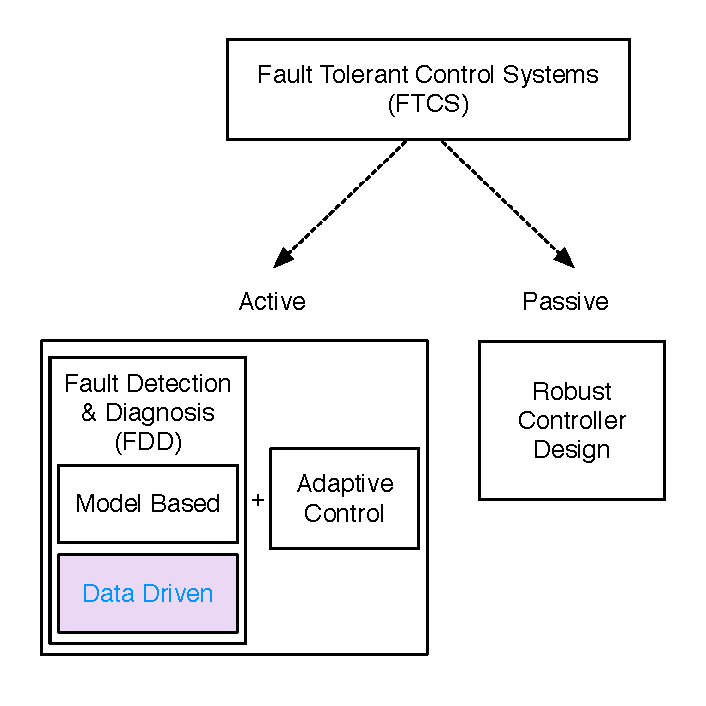
\includegraphics[width=11.3cm]{figures/FTCS}
\caption{Variations of fault tolerant control systems } 
\label{fig:FTCS}
\end{center}
\end{figure}


Even with a long list of available methods, aerospace industry has not implemented 
FTC widely, except some space systems, due to the evolving nature of the methods, 
the tricks coming with the nonlinear nature of the problem, design complexity and high 
possibility of wrong alarms in case of large disturbances and/or modeling uncertainties. 
So the already carried reliability measures concerning the hardware redundancy is 
now the preferred way because of its ease and maturity being implemented on various 
critical missions with considering human lives.

\subsection{Fault Detection and Diagnosis}

FDD is handled in two main steps; fault detection and fault diagnosis. Fault diagnosis 
encapsulates fault isolation and fault identification. The methods for detection and 
diagnosis are investigated for their frequency of utilization separately for sensor, 
actuator, process and controller faults in \cite{isermann1997trends}. FDD should 
not only be sensitive to the faults but also robust to the model uncertainties and 
external disturbances.

Two distinct options to proceed in analytical redundancy are the model based 
approaches and data-driven approaches. They form the two ends of a continuous 
solution set line, so utilizing them in a combination might end up with better solutions. 
Model based fault diagnosis highlights the components of a system and the connections 
in-between, and their corresponding fault modes. Data driven fault diagnosis rely on 
the observational data and prefers dense, redundant and with a  frequency larger than 
the failure rate. 

% This is an example of how you would use tgrind to include an example
% of source code; it is commented out in this template since the code
% example file does not exist.  To use it, you need to remove the '%' on the
% beginning of the line, and insert your own information in the call.
%
%\tagrind[htbp]{code/pmn.s.tex}{Post Multiply Normalization}{opt:pmn}

\subsubsection{Model Based Methods}

In model based approaches, relations between measurements and estimated 
states are exploited to detect possible dysfunction. The most common ways to 
implement a model based approach is to estimate the states, estimate the model 
parameters, or parity-space. The accuracy of the results depend on the type of 
faults (additive or multiplicative). Additive faults affects the variables of the process 
by a summation whereas the multiplicative faults by a multiplication.  When only 
output signal can be measured, signal model based methods can be employed for 
fault detection such as Bandpass filters, Spectral analysis(FFT) and maximum entropy estimation. 
For the case, both the input and output signals are available, the utilized methods 
for fault detection are called the process based methods: State and output 
observers(estimators), Parity equations and Identification and parameter estimation. 
They generate residuals for state variables or output variables. When previous works 
investigated, it is concluded that the most widely used technique for sensor and actuator 
faults is the state and output observers (estimators) and for process faults, identification 
and parameter estimation \cite{isermann1997trends}.

The output of the model based fault detection methods is the stochastic behaviour 
with mean values and variances. With the use of change detection methods, deviations 
from the normal behavior can be detected. For that purpose, three available methods 
considered are, mean and variance estimation, likelihood-ratio-test and Bayes decision, 
run-sum test andtwo-probe t-test. Fault detection is only supported by simple threshold 
logic or hypothesis testing in most of the applications \cite{isermann1997trends}.

A bunch of studies discovers the band of different approaches for model-based fault detection. 
Detecting sensor and actuator faults via state estimation, utilizing an EKF is applied to a 
F-16 model in \cite{hajiyev2005sensor}. Parameter identification via $H_{\infty}$ filter 
is used to indicate icing in \cite{melody2001h}.

A drawback of model-based approaches is that they require accurate model of the 
aircraft for successful detection. In a small UAV system susceptible to various 
uncertainties/disturbances and most of the cases does not have an accurate model, 
leading a model-based approach might fail. And also, a mathematical model of a UAV 
is constructed within the flight envelope, and does not necessarily describe the 
possible dynamics invoked by a failure on-board.

A way to handle that is to offer solutions to cope with the uncertainties. 
A fairly old study in 1984, investigates the design problem FDI systems robust to 
uncertainties within the models. One of the two steps of FDI, two steps being the 
residual generation and decision-making, is targeted. They offer to handle model 
uncertainties, by designing a robust residual generation process \cite{chow1984analytical}. 
Another study deals with model uncertainties by determining the threshold of the residual 
in a novel way with an application to detect aileron actuator fault \cite{rotstein2006fault}. 
\cite{sharma2007fault} utilize two cascade sliding mode observers state estimation and 
fault detection to guarantee staying in sliding manifold in the presence of unknown 
disturbances and faults. 
% This is an example of how you would use tgrind to include an example
% of source code; it is commented out in this template since the code
% example file does not exist.  To use it, you need to remove the '%' on the
% beginning of the line, and insert your own information in the call.
%
%\tgrind[htbp]{code/be.s.tex}{Block Exponent}{opt:be}

\subsubsection{Data-Driven Methods}

Model-based approaches had various successful applications until now, 
most of them assuming accurate model is available on-board. With the new 
era of UAVs, the airspace is expected to be populated by an abrupt increase 
in the number of UAVs. The variety of UAVs, expense of accurate modeling 
practices, the difficulty in modeling the behavior of UAV in case of failures, 
call for alternative approaches for the quite challenging problem of FDD. 
The increased efficiency of sensors on-board, the increase in the computational 
capabilities of autopilot processors, and the advances in machine learning 
techniques in the last decade may offer efficient data-driven solutions to FDD.

In data driven methods, a detailed knowledge about the internal dynamics 
of the system is not necessary. The data available is the source of information 
with regard to the behavior of the system. Supervised learning, which requires 
to label the fault cases previously in the training data, is usually utilized for 
data-centric inference of causes. In case of an unlabeled fault, the result is 
expected as a probability distribution of the available normal modes, identified 
fault labels and a probable unknown fault. What is needed at that point is to 
first detect and localize the fault and then to consult domain experts for labeling 
for further integration of this fault into the diagnosis scheme \cite{dataCentricDiagOffline}.

\cite{gui2002fault} argues artificial intelligent methods for fault detection of complex 
systems. Comparison between PCA and model based stochastic parity space 
approaches is given in \cite{hagenblad2004comparison}.
In \cite{li2016data}, the authors argues to use dynamic PCA since UAV flight 
controls is a dynamic system itself and DPCA can reflect unknown disturbances, 
while model-based approaches can only model typical disturbance.  

\section{Machines on the Rise}

BURAYA GECIS YAZ - authors own passion on AI + recent developments

Almost 2 decades after IBM's Deep Blue beating the chess champion Kasparov, Google DeepMind's Artificial Intelligence(AI) AlphaGo defeating 9-dan Go professional raises the question: what will be the next victory of AI?
European Parliament published a draft report with recommendations to the European Commission on Civil Law Rules on Robotics, including a list of concerns for a possible rise of the machines. 
Not only the singularity, artificial super intelligence resulting in deep changes in human civilization, but also more inevitable outcomes are discussed, such as AI's effects on workforce, ethical and legal issues inherent to automatized systems including drones.
Autonomy's effects on workforce has already been experienced, but what will be the consequences of adding more intelligence to existing automation? 
Some researchers say that, this will not lead to unemployment, but to the creation of new unforeseeable career fields, as had been the case for computer scientists after the invention of computers. 
If this is not the case, Europe is asking for solutions to cope with the imminent situation.
Until now, machine's learning processes are initiated by humans at least by giving the machine its goal. 
The community, confident that the robots will not evolve to some sort of consciousness, is referring to this fact, robots will always need humans to provide them with objectives. 
While this is debated, Google is discussing to implement a big red button to its AI DeepMind, just in case. 
The European Parliament also advices AI designers to integrate kill switches to AI. 
However, according to some experts, if an AI becomes smart enough, it might disable the kill switch and avoid such interruption. 
Although this sounds like science fiction, here we are, referencing to Isaac Asimov's laws\footnote{1. A robot may not injure a human being or, through inaction, allow a human being to come to harm. 2. A robot must obey the orders given it by human beings except where such orders would conflict with the First Law. 3. A robot must protect its own existence as long as such protection does not conflict with the First or Second Laws \cite{asimovLaws} 0. A robot may not harm humanity, or, by inaction, allow humanity to come to harm.} in documents by European Parliament \cite{civilLawRulesOnRobotics}.


Douglas Hofstadter, in his book \emph{Godel Escher Bach - An Eternal Golden Braid}, makes two analogies between: unconscious things and meaningless symbols; consciousness and patterns that are made up of these meaningless symbols. If he is right, witnessing the AI?s powers in recognizing patterns, consciousness might a probable outcome in the future. Concerns from the European Parliament is shared by popular scientists and investors such as Elon Musk, Bill Gates and Stephen Hawking. Watching Google?s humanoid robot, Atlas, running freely in the woods does not help to relieve. Opposed to the idea of this powerful tool dominated by a company or a nation, OpenAI, a nonprofit company, is aiming to distribute AI knowledge publishing open source code. Broad share of AI is also underlined in the document by European Parliament, with the proper regulations expected in the years to come.
Until then, as suggested by European Parliament, we will refer to Asimov?s Laws while designing AI:
1. A robot may not injure a human being or, through inaction, allow a human being to?come to harm.?2. A robot must obey the orders given it by human beings except where such orders would conflict with the First Law.?3. A robot must protect its own existence as long as such protection does not conflict with the First or Second Laws (See Runabout, I. Asimov, 1943)?0. A robot may not harm humanity, or, by inaction, allow humanity to come to harm.

Ref1.�http://www.europarl.europa.eu/sides/getDoc.do?pubRef=-//EP//NONSGML%2BCOMPARL%2BPE-582.443%2B01%2BDOC%2BPDF%2BV0//EN?
Ref2.�https://www.research.ibm.com/deepblue/home/html/b.html?
Ref3.�http://www.theverge.com/google-deepmind?
Ref4. HOFSTADTER, Douglas R. Godel, Escher, Bach: An Eternal Golden Braid (New York, 1979)?
Ref5.�https://www.theguardian.com/technology/2014/oct/27/elon-musk-artificial-intelligence-ai-biggest-existential-threat?
%Ref6.�https://www.theguardian.com/science/2016/oct/19/stephen-hawking-ai-best-or-worst-thing-for-humanity-cambridge?Ref7.�http://www.bbc.com/news/31047780?Ref8.�http://www.bostondynamics.com/robot_Atlas.html?
Ref9.�https://openai.com/about/?Ref10. ASIMOV, Isaac. Runaround. Astounding Science Fiction, 1942, 29.1 : 94-103.

With the last turn in popularity and practicality contest among research topics of the last decade, machine learning and drones seem to be neck to neck. The sides of the race are mostly supported by high tech rather than the public who has concerns in both opponents. Is there a chance that these two can run side by side with cheers? Machine learning guides various aspects of our lives even without noticing it due to its abrupt introduction via the bigger tech companies. Its abilities rise, defeating 9-dan Go professional, their accuracy increase, enabling smooth voice recognition, adding intelligence to our daily lives. Another machine, who wants to enjoy this enabling technology is a drone. Drones, although still very strictly regulated in most countries have been spreading with great passion along their enthusiasts. Machine learning has already started to take part in aviation. Operational improvements on aviation is one of the preliminary fields it appeared. Recently an AGE sponsored competition for data scientists resulted in the first place award with \%12 improvement in fuel consumption efficiency by the designed routing algorithm from real flight data. Some other operational problems issued by machine learning are accurate arrival time estimation and calculating optimal parameters for take off, mostly for reducing the cost of the airlines and increasing customer satisfaction. Yet another application is to deal with the expected shortage of pilots, inevitable in the years to come, thanks to the increasing demand for air travel. So a��prospective utilization of machine learning is to assess the competency of pilots with unsupervised learning models in order to reduce the long duration of pilot training, hence contributing to tackle pilot shortage problem. Use of data-driven approaches for pilot training could be used not only for assessment of the pilots but also to increase the efficiency of the training by offering trainee focused personal training, adapting the curriculum to their individual skills and needs. To overcome the pilot shortage, another way to handle the problem might be to reduce the need for one. One of the goals of the autonomy researchers is to look for ways to implement artificial intelligence to one of the core features of an aircraft: the autopilot. Hence the ability to use them is tricky due to the inherent nature of the methods, non-determinism. EASA A-NPAs offer different categories to enjoy for drones, depending on the risk of the operation of concern. The difficulties waiting the machine learning researches are not really well defined or widely argued in aviation. In this paper, we offer to present the challenges and discuss the possible paths to offer machine learning algorithms to have a wider role in aviation. AI has actually already sneaked into the cockpit. Garmin implemented voice recognition features garnished with some other functions such as changing radio channels to aid the pilots with its audio panels GMA 350 and GMA 35, called ?Telligence?. We aim to discuss the enablers and try to understand the borders that might result or prevent the similar fate of machine learning implementations on safety systems onboard, widely referring to the AIAA Roadmap for Intelligent Systems.


